\documentclass[a4paper,12pt,twocolumn,oneside,openright,final]{memoir}
\usepackage[english]{babel}
\usepackage{etex}
\usepackage{times}
\usepackage{setspace}
\usepackage{inputenc}
\usepackage{amssymb}
\usepackage{amsfonts}
\usepackage[pdftex]{graphicx}
%\usepackage{subfigure}
\usepackage{alltt}
\usepackage{moreverb}
%for more info on hyperref package see http://en.wikibooks.org/wiki/LaTeX/Packages/Hyperref
\usepackage[pdftex,colorlinks=true,linkcolor=blue]{hyperref}
\usepackage{eso-pic}
\usepackage{transparent}
\setlength{\columnsep}{3em}

\usepackage{wrapfig}
\usepackage{subfig}
\usepackage{alltt}
\usepackage{moreverb}
% tikz related packages to provide scalable graphics 
\usepackage{tikz}
\usetikzlibrary{calc,mindmap,backgrounds,positioning,arrows,shapes,shapes.arrows,shapes.misc,automata,petri,patterns,scopes,chains,matrix,decorations.pathmorphing,shadows,calc}


\usepackage{geometry}
%\geometry{hmargin={30mm,15mm},vmargin={26mm,26mm}}
%\geometry{total={14cm,20.5cm},includehead}
\geometry{hmargin={15mm,15mm},vmargin={20mm,20mm}}

\usepackage[pages=some]{background}

\backgroundsetup{
  scale=1.2,
  angle=0,
  opacity=0.4,
  contents={
    
\includegraphics[width=1.1\paperwidth,height=1.1\paperheight, keepaspectratio]{images/00-background.png}} 
}


%\AddToShipoutPicture{
%\put(0,0){
%	\parbox[b][\paperheight]{\paperwidth}{%
%		\vfill
%		\centering
%		{\transparent{0.1}
\includegraphics[width=1.1\paperwidth,height=1.1\paperheight, keepaspectratio]{images/00-background.png}}%
%		\vfill
%		}
%	}
%}

\begin{document}
\BgThispage
\subsection*{What is TG?}
  Trident Genesis (TG) is an opinionated software development platform for development of information systems in a domain driven way.
  It lifts up the level of abstraction to the modelling of the business domain, while automatically handling low level technical details.
  
  \vspace{5 mm}
  \noindent The architecture of the business domain is often unique. 
  This what makes companies competitive.
  Modelling the business domain as a software information systems that facilitate the business lifecycle is the core value for customers.
  
  \vspace{5 mm}
  \noindent The TG platform incorporates over 30 years of experience in delivering Enterprise grade software solutions at a software architecture level.
  It encapsulates the complexity of the low technical details for efficient database communication, concurrent data processing, HTML5 client construction to enable software developers concentrate on the business domain architecture.


  \begin{figure}[!h]
    \vspace{0pt}
    \centering   
    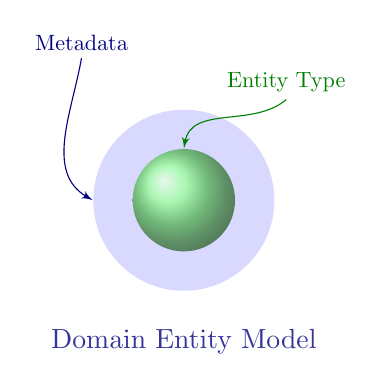
\begin{tikzpicture}[>=latex']
      \tikzset{
	  outercore/.style={circle, fill=blue!50!white, inner sep=0em, minimum size=2.3cm},
	  core/.style={circle, shade, ball color=green!50!white, inner sep=0em, minimum size=1.3cm},
      }      
      \begin{scope}[opacity=0.8]
	\node (o) at (0, 0) [outercore, opacity=0.3] {};	
	\node (c) at (0, 0) [core] {};
	\node at (0, -1.8cm) [text=blue!50!black] {Domain Entity Model};
      \end{scope}

      \node (ot) at (1.3, 1.5) [text=green!50!black,scale=0.8] {Entity Type};	
      \fill [green!50!black,->,out=220,in=80] (ot.south) edge (c.north);
      \node (ct) at (-1.3, 2) [text=blue!50!black,scale=0.8] {Metadata};	
      \fill [blue!50!black,->,out=-100,in=150] (ct.south) edge (o.west);      
    \end{tikzpicture} 
    \vspace{-10pt}
  \end{figure}

  \noindent The typical development workflow includes: modelling of the business domain (declarative ontological aspect), implementing core business rules (imperative aspect) and configure the user interface.
  These steps are facilitated by high level abstractions provided by the platform.
  The platform enables developers to concentrate on the modelling of the business domain. 
  This ensures higher productivity, quality and value of the final software system to the business.

    \begin{figure}[!h]
    \vspace{0pt}
    \centering    
    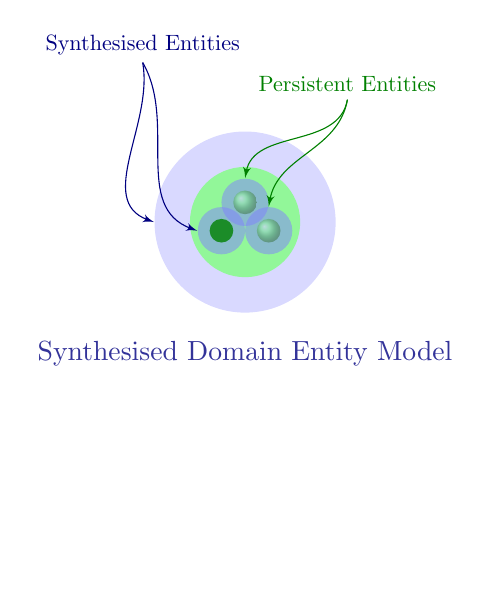
\begin{tikzpicture}[>=latex']
      \tikzset{
	  outercore/.style={circle, fill=blue!50!white, inner sep=0em, minimum size=0.6cm},
	  core/.style={circle, shade, ball color=green!50!white, inner sep=0em, minimum size=0.3cm},
	  score/.style={circle, fill=green!50!black, inner sep=0em, minimum size=0.3cm},
	  outer/.style={circle, fill=blue!50!white, inner sep=0em, minimum size=2.3cm},
      }
      \begin{scope}[opacity=0.8]
	\node (o) at (0, -0.25) [outer, opacity=0.3] {};      
	\fill[circle, color=green!50!white] (0, -0.25) circle (0.7cm) node [below,text=blue!50!black,yshift=1.1cm] {Synthesised Domain Entity Model};
      \end{scope}
      
      \begin{scope}[scale=0.3,opacity=0.8]
	\node (t) at (0,0) [outercore, opacity=0.5] {};	
	\node at (0,0) [core, opacity=0.5] {};

	\node (r) at (1,-1.2) [outercore, opacity=0.5] {};	
	\node at (1,-1.2) [core, opacity=0.5] {};

	\node (l) at (-1,-1.2) [outercore, opacity=0.5] {};	
	\node at (-1,-1.2) [score] {};
      \end{scope}
      
      \node (pe) at (1.3, 1.5) [text=green!50!black,scale=0.8] {Persistent Entities};      
      \fill [green!50!black,->,out=-100, in=80] (pe.south) edge (t.north);
      \fill [green!50!black,->,out=-100,in=80] (pe.south) edge (r.north);
      
      \node (se) at (-1.3, 2) [text=blue!50!black,scale=0.8] {Synthesised Entities};
      \fill [blue!50!black,->,out=-60,in=160] (se.south) edge (l.west);
      \fill [blue!50!black,->,out=-80,in=160] (se.south) edge (o.west);      
    \end{tikzpicture} 
    \vspace{-75pt}
  \end{figure}


 \subsection*{Core Principles and Advantages}
  TG is designed to ensure that the application facilitates communication between different business stakeholders and is easy to use by incorporates the following principles and approaches:

  \begin{itemize}
    \item Unique object-oriented architectural style to uniform modelling of the business domain.
    \item Optimised for relational databases.
    \item Direct interaction and manipulation of the business model from UI for data interrogation, analysis and reporting.
    \item Automated business model verification through domain driven testing.
    \item Continuous validation of the business models during the system lifecycle.
    \item Two-factor authentication (SMS, emails).
    \item Declarative authorisation with pluggable backends (e.g. LDAP). 
    \item Secure HTTPS communication as a standard.
    \item Responsive HTML5 client side, which follows Google Material Design principles.
    \item Complete application development lifecycle (from business model to database to UI).
    \item Cloud ready.
    \item Single programming language (Java).
   \end{itemize}

  \begin{figure}[!h]
  \centering
  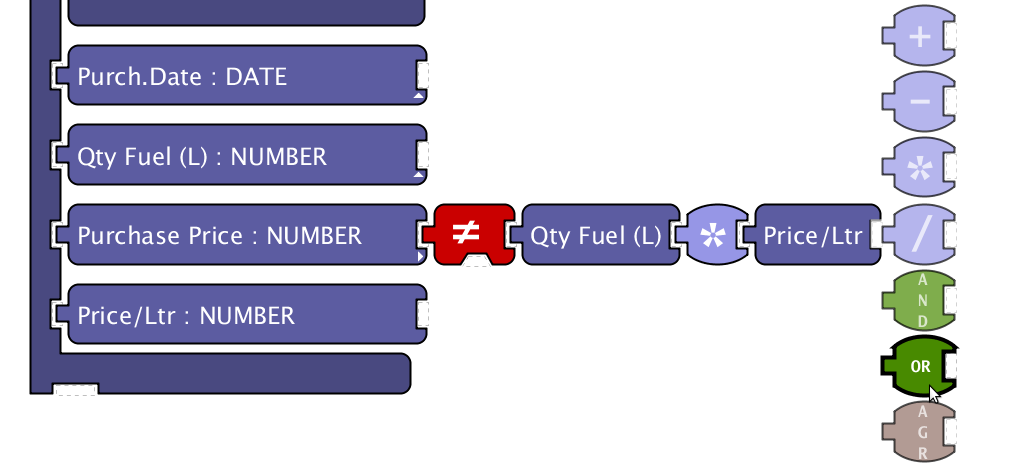
\includegraphics[scale=0.22]{images/01-rulesarea-suggestionmenu.png}  
  \end{figure}

\subsection*{Designed for ease of use and learning by end-users and developers alike}

\subsubsection*{Development Model}
  Platform ensures that all TG-based applications follow exactly the same development model leading to structural and behavioural uniformity.
  This protects developers from multitude of programming errors provisioning for getting a working solution in short terms, which can be easily supported by the original or new developers.

\BgThispage
 
\subsubsection*{Intuitive}
  From constant communication with customers, Fielden understands how their applications are utilised. 
  We incorporate this understanding into the ways TG-based applications are designed covering task flows and features that are essential at key points within the user experience, making the application extremely intuitive.
  Applications always provide a sensible feedback to the user in non-intrusive ways reducing the confusion and disruption of the workflow.
  \begin{figure}[!h]
  \centering
  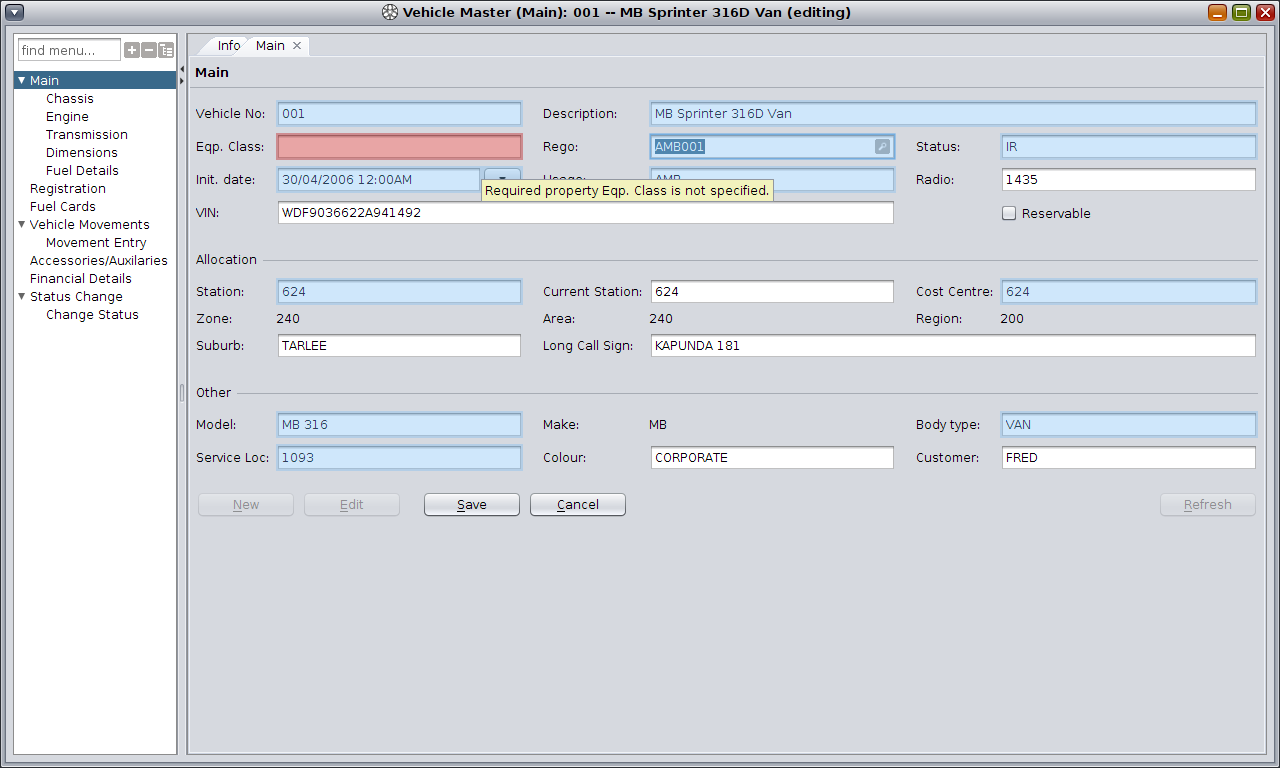
\includegraphics[scale=0.17]{images/04-veh-master-main-error.png}
  \end{figure}

\subsubsection*{Consistency}

  Consistency makes software easier to use. 
  Things that look the same should behave in a consistent fashion, and an action should always produce the same result. 
  In TG-based applications, all UI elements that look the same -- operate the same way. 
  The platform provides the highest level of consistency across all parts of the application to quickly move from function to function, without confusion and wasted effort.
 
\subsubsection*{Flexibility}
  Recognising that every customer and every user is different, TG platform is designed to provide high flexibility of the end product. 
  Organisations using TG-based solutions do not have to change processes or terminology -- their domain is fully reflected in the application. 
  Users can customise the application to meet their unique needs.
  The administrative function provides easy ways to configure and customise access to the features that users should access based on their role.

  \begin{figure}[!h]
  \centering
  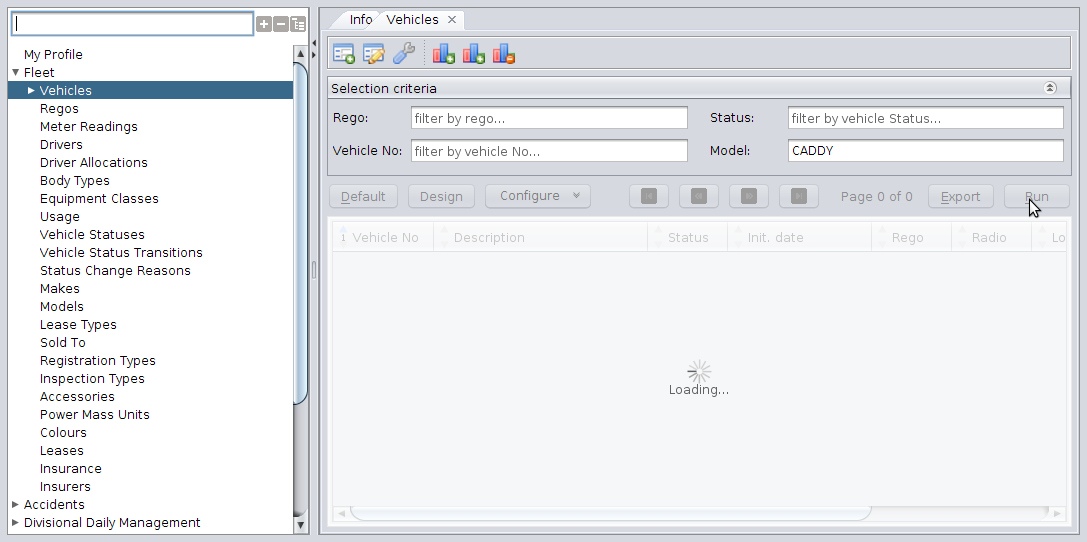
\includegraphics[scale=0.2]{images/03-running.png}
  \end{figure}

\subsubsection*{Interactivity}
  TG-based applications utilise the full potential and richness of the desktop UI providing users with highly interactive experience.
  The platform incorporates the implementation of the Zooming User Interface paradigm, which provides support for integration with Scalable Vector Graphics files.

  \begin{figure}[!h]
  \centering
 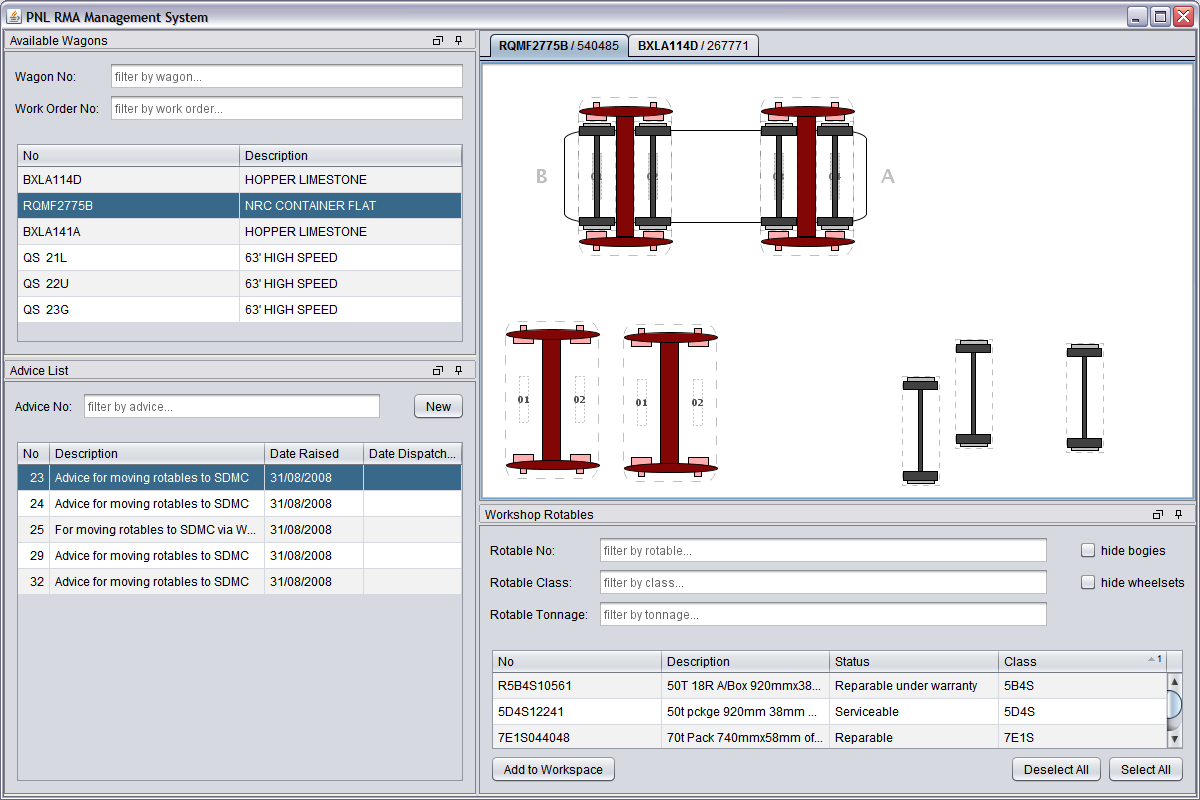
\includegraphics[scale=0.18]{images/02-workspace-custom-layout.png}
  \end{figure}

\subsubsection*{Cloud \& Scalability}
  Due to the platform's stateless Resource Oriented Architecture and intelligent data processing, TG-based applications are highly scalable (no need to manage server-side state) and well suited to operate on computer clusters and cloud infrastructures such as Amazon EC2.

\end{document}

